\documentclass[12pt,a4paper]{article}
% Estilo compartido para informes. Compilar con LuaLaTeX desde tp1/.
\usepackage[spanish,es-nodecimaldot]{babel}
\usepackage{fontspec}
\setmainfont{Montserrat-Medium.ttf}[
  Path=../assets/fonts/,
  BoldFont=Montserrat-Bold.ttf,
  ItalicFont=Montserrat-MediumItalic.ttf]
\usepackage[a4paper,margin=2.5cm,headheight=16pt]{geometry}
\usepackage{xcolor,graphicx,booktabs,tabularx}
\usepackage{float}
\usepackage{titlesec,fancyhdr,enumitem,caption}
\usepackage{ragged2e}
\usepackage{hyperref}
\definecolor{verde}{HTML}{1D4036}
\definecolor{bronce}{HTML}{D38129}
\definecolor{rosa}{HTML}{D88E77}
\definecolor{calido}{HTML}{EFE4D8}
\definecolor{grafito}{HTML}{1D1D1D}
\hypersetup{colorlinks=true,linkcolor=verde,urlcolor=verde,
  pdftitle={TP1 - Instalación de máquinas virtuales},pdfsubject={Cyberseguridad}}
\AtBeginDocument{\color{grafito}\RaggedRight\fontsize{12}{14.4}\selectfont}
\setlength{\parindent}{0pt}
\setlength{\parskip}{7pt}
\setlist[itemize]{leftmargin=*,itemsep=7pt,topsep=4pt}
\setlist[enumerate]{leftmargin=*,itemsep=6pt}
\titleformat{\section}{\color{verde}\bfseries\fontsize{18}{21.6}\selectfont}{\thesection}{0.65em}{}
\titleformat{\subsection}{\color{verde}\bfseries\large}{\thesubsection}{0.65em}{}
\titleformat{\subsubsection}{\color{verde}\bfseries}{\thesubsubsection}{0.65em}{}
\titlespacing*{\section}{0pt}{16pt}{8pt}
\titlespacing*{\subsection}{0pt}{12pt}{5pt}
\titlespacing*{\subsubsection}{0pt}{10pt}{4pt}
\setcounter{tocdepth}{2}
\pagestyle{fancy}
\fancyhf{}
\fancyhead[L]{\small\color{verde}FCEFyN | UNC}
\fancyhead[R]{\small\color{verde}\materia\ · TP \numeroTP}
\fancyfoot[L]{\scriptsize Informe de laboratorio}
\fancyfoot[R]{\small\thepage}
\renewcommand{\headrulewidth}{0.4pt}
\captionsetup{font=small,labelfont=bf,justification=raggedright,singlelinecheck=false,hypcap=false}
\newcommand{\pendiente}[1]{\par{\small\color{verde}\textbf{Por completar.} #1\par}}
% Si falta una captura se muestra un espacio reservado; no impide compilar.
\newcommand{\captura}[2]{%
  \par\smallskip\begingroup\centering
  \IfFileExists{figuras/#1}{%
    \includegraphics[width=\linewidth,height=5cm,keepaspectratio]{figuras/#1}%
  }{%
    \setlength{\fboxsep}{10pt}%
    \fcolorbox{bronce}{calido}{\parbox[c][1.25cm][c]{\dimexpr\linewidth-2\fboxsep-2\fboxrule\relax}{%
      \centering\small Captura pendiente\par\texttt{\detokenize{#1}}}}%
  }%
  \captionof{figure}{#2}\par\endgroup\smallskip
}

\usepackage{xurl}

\newcommand{\materia}{Cyberseguridad}
\newcommand{\numeroTP}{14}
\newcommand{\tituloTP}{Control de acceso SSH y MFA}
\newcommand{\estudiante}{Brigido Tomas Andres}
\newcommand{\legajo}{38481096}
\newcommand{\carrera}{ICOMP}
\newcommand{\docente}{Javier A. Jorge}


% Metadatos específicos del TP14 y capturas en img/.
\hypersetup{pdftitle={TP14 - Control de acceso SSH y MFA},linkcolor=black,urlcolor=black,citecolor=black}
\renewcommand{\captura}[2]{%
  \begin{figure}[H]
    \centering
    \IfFileExists{img/#1}{%
      \includegraphics[width=0.85\linewidth,height=5cm,keepaspectratio]{img/#1}%
    }{%
      \setlength{\fboxsep}{10pt}%
      \fcolorbox{bronce}{calido}{\parbox[c][1.1cm][c]{0.85\linewidth}{%
        \centering\small Captura pendiente\par\texttt{\detokenize{#1}}}}%
    }%
    \caption{#2}
  \end{figure}
}

\usepackage{caption}
\captionsetup{justification=centering}
\begin{document}
\hypersetup{pageanchor=false}
\begin{titlepage}
  
\includegraphics[width=8cm]{../assets/logo-fcefyn-2026.png}
  \vspace{1cm}

  {\color{verde}\small UNIVERSIDAD NACIONAL DE CÓRDOBA\par}
  \vspace{2.1cm}
  {\color{bronce}\bfseries\large TRABAJO PRÁCTICO \numeroTP\par}
  \vspace{0.45cm}
  {\color{verde}\bfseries\fontsize{32}{38.4}\selectfont Control de acceso\\SSH y MFA\par}
  \vspace{0.3cm}
{\small Claves, autorización y autenticación multifactor\par}
\vspace{0.35cm}
  {\large \materia\par}
  \vspace{0.8cm}
  {\color{bronce}\rule{2.7cm}{2pt}\par}
  \vfill
  \renewcommand{\arraystretch}{1.45}
  \begin{tabular}{@{}p{3.2cm}p{10cm}@{}}
    Estudiante & \estudiante \\
    Legajo & \legajo \\
    Carrera & \carrera \\
    Docente & \docente \\
  \end{tabular}
  \vfill
  {\small Córdoba, Argentina\par}
\end{titlepage}
\hypersetup{pageanchor=true}

\tableofcontents
\vspace{1cm}
\newpage

\section{Introducción y objetivos}
Se configuró el acceso SSH a una VM Debian mediante claves públicas y privadas, autorización con PAM y códigos TOTP. También se evaluó la detección de intentos fallidos con Fail2ban.

\section{Acceso SSH mediante claves}
\subsection{Generación de claves y agente SSH}
Se generó un par de claves Ed25519 mediante \texttt{ssh-keygen}. La clave privada se guardó como \texttt{clave prueba} y la pública como \texttt{clave prueba.pub}. Luego se consultó el contenido de la clave pública con \texttt{cat}.
\captura{ssh-key-generada.png}{Generación del par de claves Ed25519.}
\captura{key-publica.png}{Archivos generados y contenido de la clave pública.}
\par\textbf{¿Cuáles son los algoritmos que puede utilizar SSH? ¿RSA sigue vigente?}

Para autenticación por claves, SSH admite Ed25519, ECDSA y RSA, entre otros. RSA sigue vigente con firmas SHA-2; la variante antigua \texttt{ssh-rsa}, que utiliza SHA-1, está deshabilitada por defecto en OpenSSH moderno.
% Fuente: https://www.openssh.org/releasenotes.html

\newpage
\subsection{Conexión inicial y autorización de la clave}
Se activó el servidor SSH en la VM y se ingresó con el usuario \texttt{osboxes} mediante contraseña. Se utilizó \texttt{ssh -p 2222 osboxes@127.0.0.1}, con un reenvío de puertos de VirtualBox desde el puerto 2222 del host hacia el puerto 22 de la VM (\texttt{10.0.2.15}).
\begin{figure}[H]
    \centering
    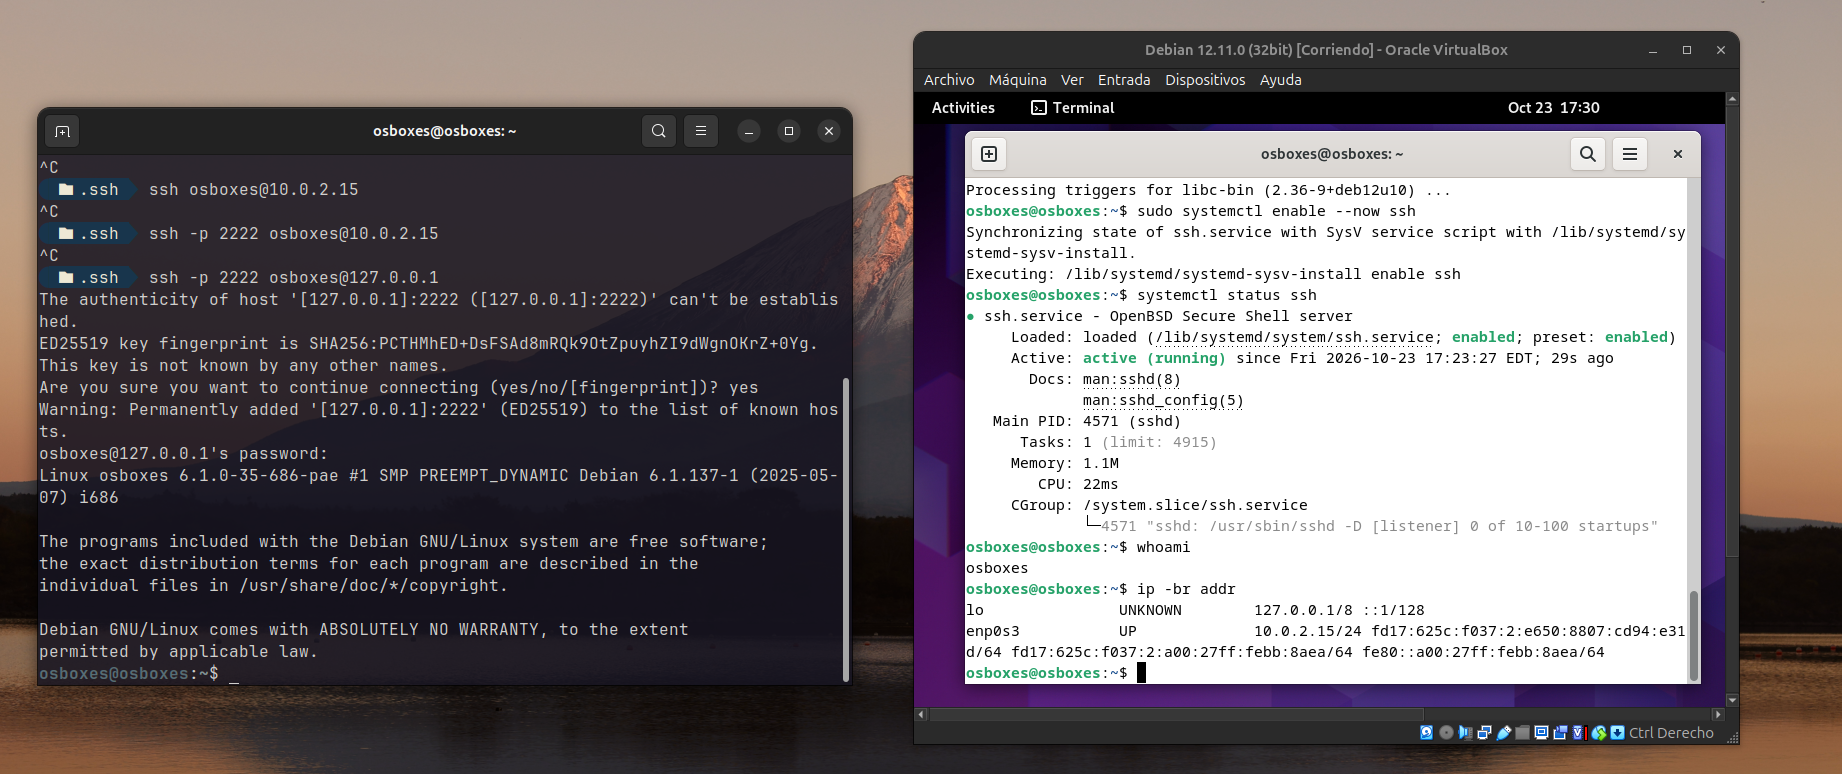
\includegraphics[width=\linewidth]{img/conexion-por-ssh-vm.png}
    \caption{Servidor SSH activo en la VM y conexión desde el host con el usuario osboxes.}
\end{figure}
\par\textbf{¿Puede ingresar con root? ¿Por qué?}

No se comprobó el acceso como root: la captura muestra el ingreso como \texttt{osboxes}. El acceso de root depende de la configuración del servidor SSH y del método de autenticación permitido.

Se copió la clave pública al servidor mediante \texttt{ssh-copy-id} y se comprobó su presencia en \texttt{\detokenize{~/.ssh/authorized_keys}}. Tras un primer intento con un error del agente SSH, se logró una nueva conexión sin que se solicitara la contraseña del usuario.
\begin{figure}[H]
    \centering
    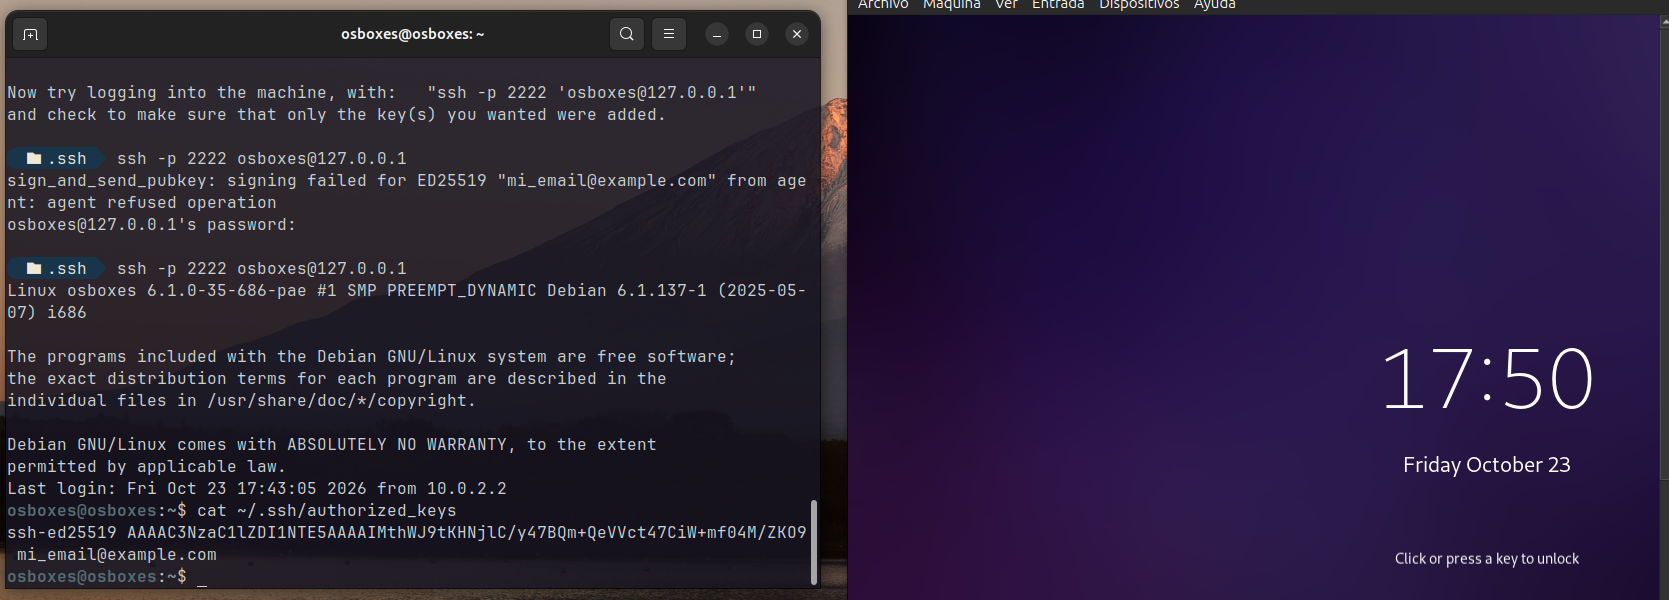
\includegraphics[width=\linewidth]{img/publikey-en-debian.png}
    \caption{Conexión SSH y comprobación de la clave pública en authorized\_keys.}
\end{figure}

\newpage
\subsection{Acceso sin contraseña de cuenta y nuevo usuario}
Se modificó \texttt{/etc/ssh/sshd\_config} para establecer \texttt{PasswordAuthentication no} y deshabilitar la autenticación por contraseña.
\begin{figure}[H]
    \centering
    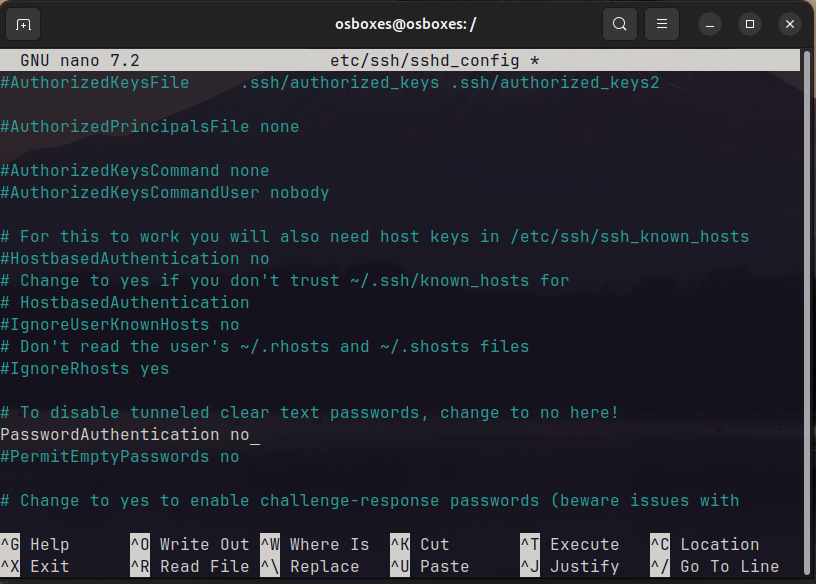
\includegraphics[width=0.63\linewidth]{img/password-authentication-no.png}
    \caption{Desactivación de la autenticación por contraseña en SSH.}
\end{figure}
Se creó el usuario \texttt{nopriv} en la VM y se probó el acceso desde el host con \texttt{ssh -p 2222 nopriv@127.0.0.1}. El servidor rechazó la conexión por falta de una clave autorizada.
\begin{figure}[H]
    \centering
    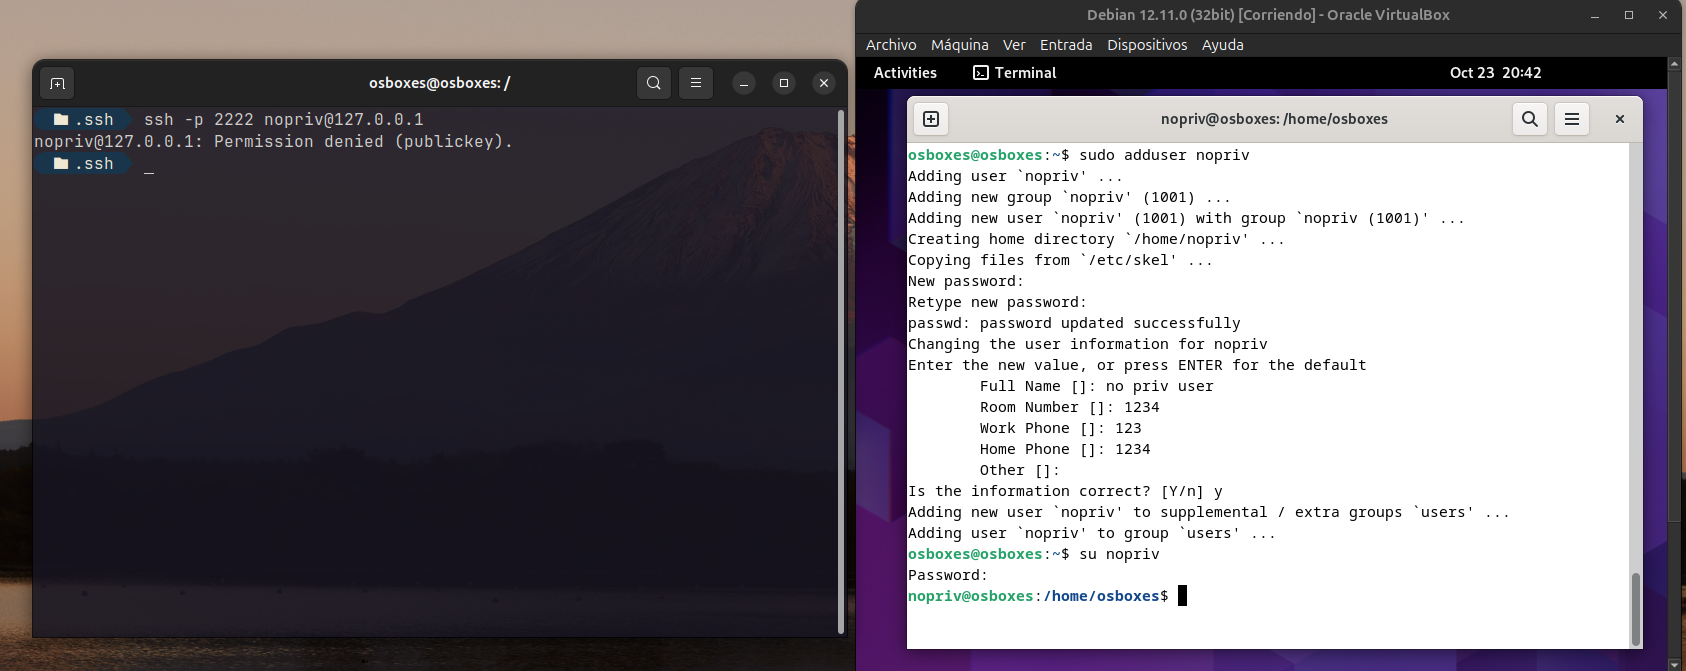
\includegraphics[width=\linewidth]{img/nuevo-usuario.png}
    \caption{Creación de nopriv y rechazo de su conexión SSH.}
\end{figure}
\par\textbf{¿Puede ingresar? ¿Por qué? ¿Cómo podemos hacer para poder ingresar?}

No puede ingresar porque no tiene una clave pública autorizada y el servidor exige autenticación por clave. Para permitir el acceso, se debe agregar nuestra clave pública a \texttt{/home/nopriv/.ssh/authorized\_keys}, con propietario y permisos adecuados.

\newpage
\subsection{Ubicación de claves autorizadas y banner}
\texttt{AuthorizedKeysFile} indica dónde busca SSH las claves públicas autorizadas de cada cuenta. En esta práctica se utilizó \texttt{\detokenize{~/.ssh/authorized_keys}}, sin trasladar las claves a una ubicación centralizada.

Se configuró un banner de bienvenida con un aviso de acceso autorizado. Al iniciar una nueva conexión SSH, se comprobó que el mensaje se muestra correctamente.
\begin{figure}[H]
    \centering
    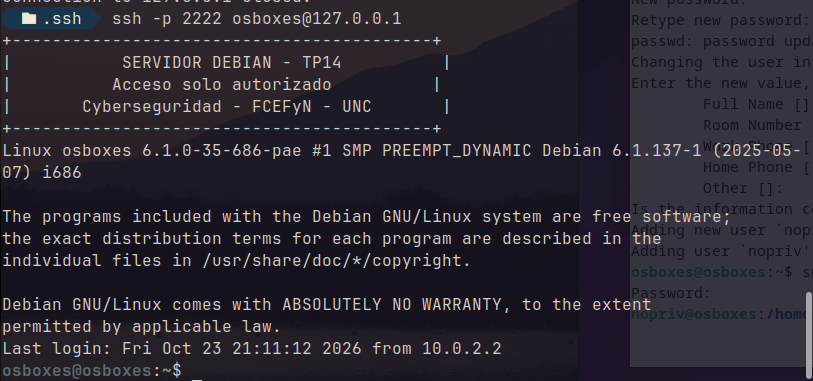
\includegraphics[width=\linewidth]{img/banner.png}
    \caption{Banner presentado al conectarse por SSH.}
\end{figure}

\newpage
\section{Ampliaciones de protección SSH (opcionales)}
\subsection{Autorización con PAM}
Se agregó el usuario \texttt{osboxes} a \texttt{/etc/ssh/ssh.deny} y se configuró PAM con el módulo \texttt{pam\_listfile} para denegar su acceso. SSH se configuró para exigir clave pública y autenticación interactiva mediante PAM.

La conexión fue rechazada y los registros mostraron \texttt{Refused user osboxes for service sshd}, confirmando que PAM bloqueó el acceso de esa cuenta.
\begin{figure}[H]
    \centering
    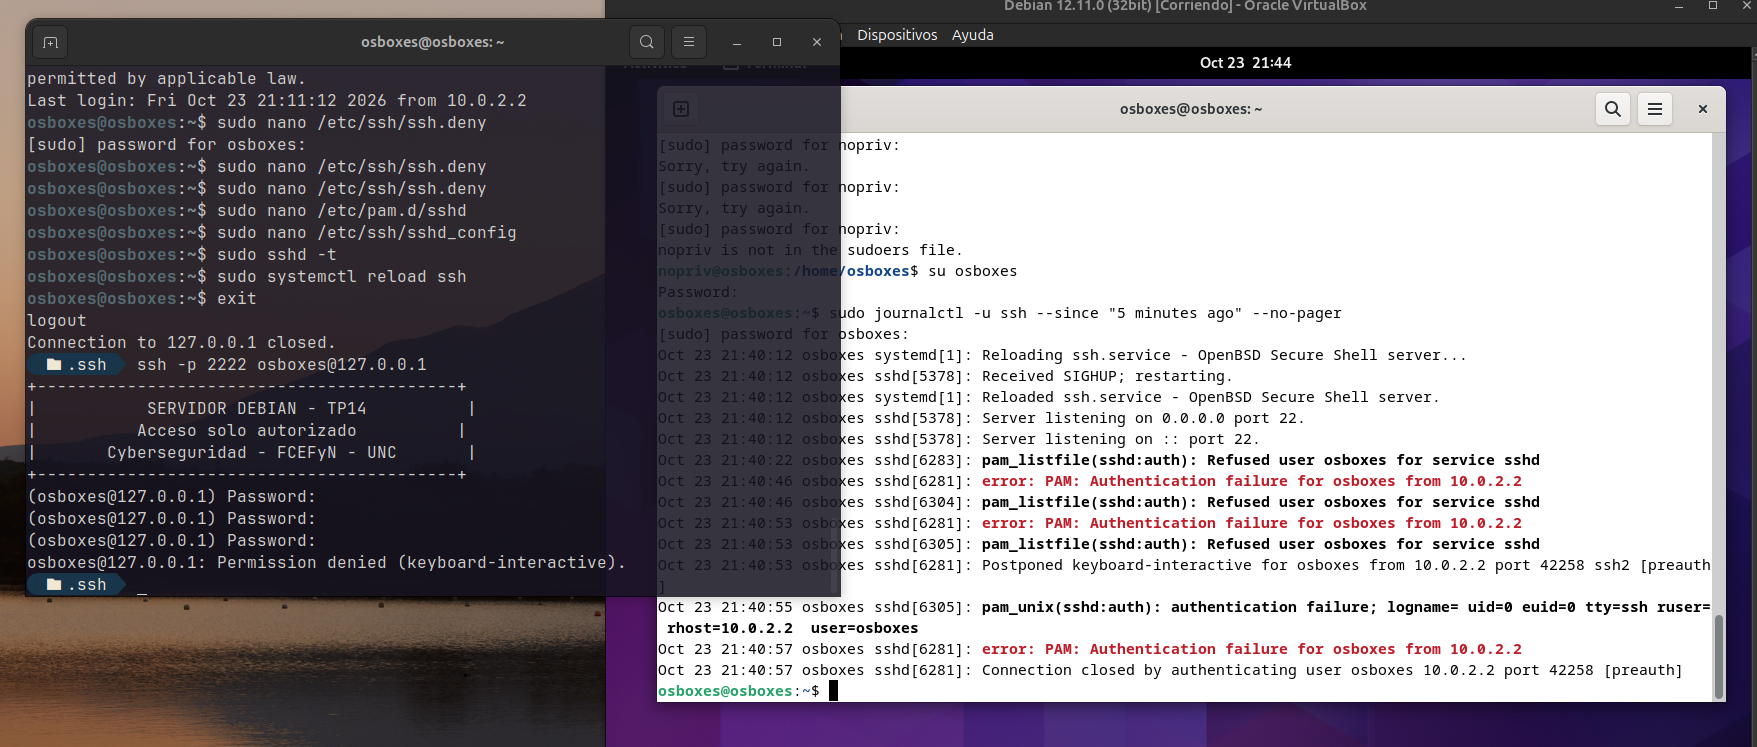
\includegraphics[width=\linewidth]{img/PAM.png}
    \caption{Rechazo de la conexión SSH y registros del bloqueo de osboxes mediante PAM.}
\end{figure}

\newpage
\subsection{Fail2ban}
Se realizaron intentos de acceso SSH con contraseñas incorrectas y se consultó el estado de Fail2ban mediante \texttt{sudo fail2ban-client status sshd}.
\par\textbf{Intente ingresar con la contraseña equivocada múltiples veces. ¿Qué sucede? ¿Cuál es la salida del comando ``sudo iptables -L''?}

Fail2ban registró siete fallos y marcó la IP \texttt{10.0.2.2} como bloqueada. Sin embargo, luego se pudo ingresar con la contraseña correcta, por lo que no se confirmó un bloqueo efectivo. No se obtuvo la salida de iptables: el comando no fue encontrado.
\begin{figure}[H]
    \centering
    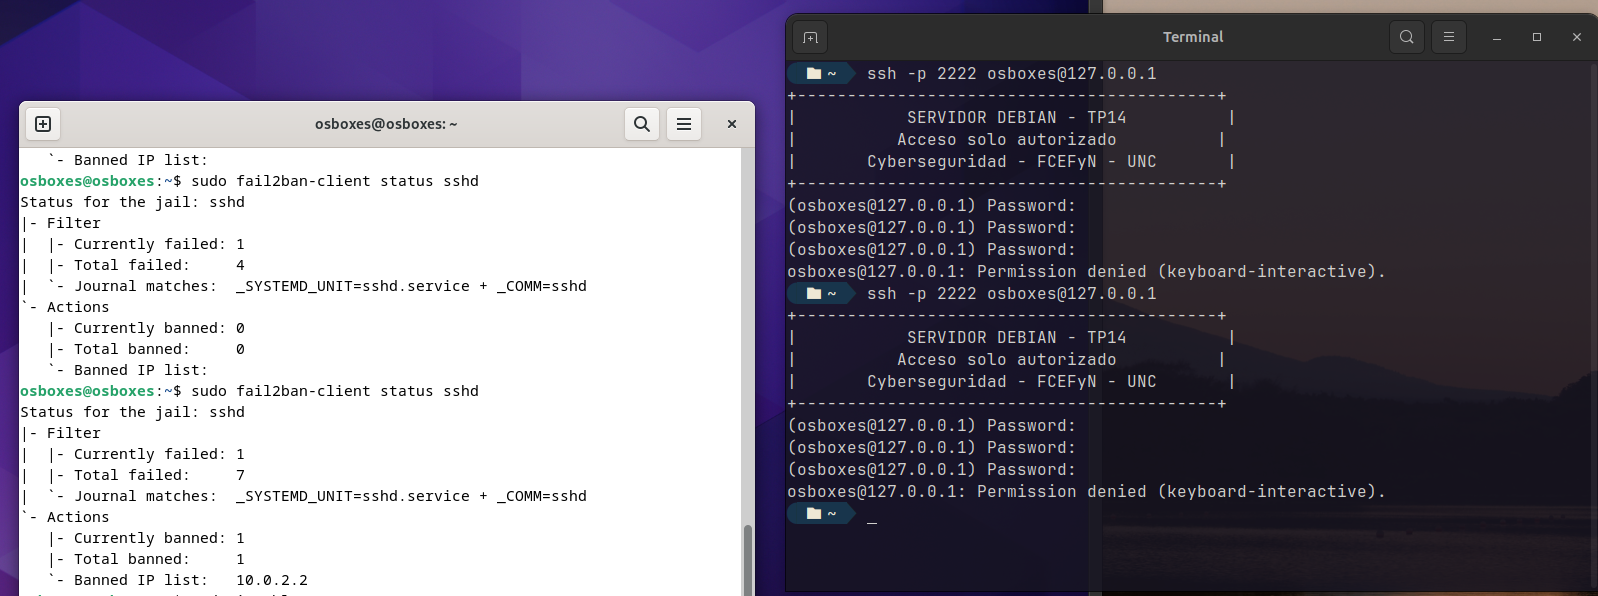
\includegraphics[width=\linewidth]{img/baned-ip.png}
    \caption{Intentos fallidos e IP marcada como bloqueada por Fail2ban.}
\end{figure}

\subsection{Reflexión}
\par\textbf{¿En qué casos conviene listar los usuarios a denegar el acceso? ¿Sería más interesante listar solamente a quienes deseo permitir el acceso? ¿En qué casos puede tener sentido?}

Una lista de denegados sirve para excluir cuentas puntuales. Una lista de permitidos es conveniente cuando solo un grupo reducido debe acceder, ya que rechaza al resto por defecto.
\par\textbf{¿Qué otros servicios puede vigilar Fail2ban? ¿Se puede configurar para que envíe alertas cuando se active?}

Puede vigilar servicios como servidores web, FTP y correo, mediante filtros de sus registros. También puede enviar alertas por correo si se configura la acción de notificación y el servicio de envío.

\newpage
\section{Autenticación multifactor en SSH}
\subsection{Preparación del segundo factor}
Se instaló \texttt{libpam-google-authenticator} y se ejecutó \texttt{google-authenticator} como \texttt{osboxes}, sin sudo. Se vinculó la cuenta con Google Authenticator mediante un QR para generar códigos temporales TOTP. Se configuró la prohibición de reutilizar códigos, la ventana temporal predeterminada y la limitación de intentos.

\subsection{Integración con SSH y PAM}
En \texttt{/etc/pam.d/sshd} se comentó \texttt{@include common-auth} y se agregó esta regla:
\begin{verbatim}
auth required pam_google_authenticator.so
\end{verbatim} Así, PAM verifica el código temporal en lugar de la contraseña del usuario. Se retiró a \texttt{osboxes} de la lista de denegados para permitir su acceso.

En \texttt{/etc/ssh/sshd\_config} se mantuvo la siguiente configuración:
\begin{verbatim}
PubkeyAuthentication yes
PasswordAuthentication no
KbdInteractiveAuthentication yes
UsePAM yes
AuthenticationMethods publickey,keyboard-interactive
\end{verbatim}
La conexión exige validar la clave SSH y luego el código TOTP del celular.

\newpage
\subsection{Pruebas de acceso}
Al conectarse desde el host, SSH solicitó \texttt{Verification code}. Después de ingresar el código del autenticador, se inició la sesión de \texttt{osboxes}. No se documentó una prueba con un código TOTP incorrecto.
\begin{figure}[H]
    \centering
    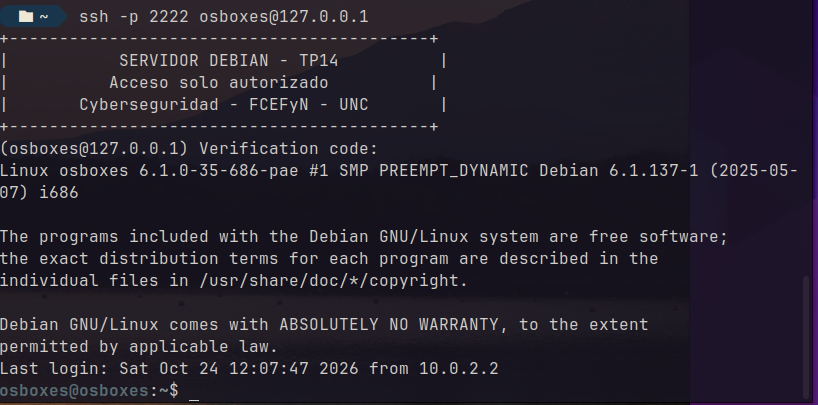
\includegraphics[width=\linewidth]{img/authenticator.png}
    \caption{Solicitud del código TOTP e ingreso exitoso a la VM.}
\end{figure}

\clearpage
\section{Conclusión}
Se comprobó el acceso por claves, el rechazo de usuarios mediante PAM y el ingreso con clave SSH y código TOTP. Fail2ban detectó fallos y registró una IP bloqueada, aunque no se confirmó la aplicación efectiva del bloqueo en el firewall.

\clearpage
\section{Referencias}
\begin{itemize}
    \item \textit{Control de acceso usando SSH y técnicas de protección}. Consigna de laboratorio provista por la cátedra.
    \item \textit{Multi-factor authentication (MFA)}. Consigna de laboratorio provista por la cátedra.
\end{itemize}
\end{document}
